\documentclass[margin=10pt]{standalone}
\usepackage{tikz}

\usetikzlibrary{calc, intersections, decorations.markings}

\begin{document}

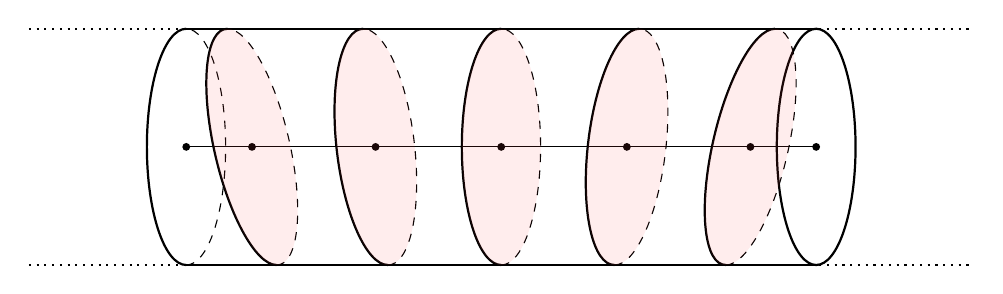
\begin{tikzpicture}
  \tikzset{
    partial ellipse/.style args={#1:#2:#3}{
      insert path={+ (#1:#3) arc (#1:#2:#3)}
    }
  }

  \pgfmathsetmacro{\xmin}{-4}
  \pgfmathsetmacro{\xmax}{4}

  % For the dotted lines extending the tube
  \pgfmathsetmacro{\xminext}{\xmin - 2}
  \pgfmathsetmacro{\xmaxext}{\xmax + 2}

  % The minor (? I forgot what it's called ?) axis diameter
  \pgfmathsetmacro{\minorx}{.5}

  \pgfmathsetmacro{\ymin}{-1.5}
  \pgfmathsetmacro{\ymax}{1.5}


  \draw[thick] (\xmax,0) ellipse (\minorx cm and \ymax cm);
  \draw[thick] (\xmin,0) [partial ellipse=90:270:\minorx cm and \ymax cm];
  \draw[dashed] (\xmin,0) [partial ellipse=-90:90:\minorx cm and \ymax cm];

  \draw (\xmax,0) -- (\xmin, 0);
  \node[fill=black, inner sep=1pt, circle] () at (\xmax,0) {};
  \node[fill=black, inner sep=1pt, circle] () at (\xmin,0) {};



  \draw[thick] (\xmin,\ymin)--(\xmax,\ymin);
  \draw[thick] (\xmin,\ymax)--(\xmax,\ymax);
  \draw[thick, dotted] (\xminext,\ymin)--(\xmaxext,\ymin);
  \draw[thick, dotted] (\xminext,\ymax)--(\xmaxext,\ymax);

  % Associated ellipse
  % Takes as arg: how far along the tube to draw the center of our
  % ellipse (-1 for left endcap, 1 for right endcap)
  \def\asscellipse#1{
    % shear angle
    %
    % 30 is maximum shear angle
    \pgfmathsetmacro{\shear}{#1*30}
    \pgfmathsetmacro{\xshift}{#1*4}

    \begin{scope}[cm={cos(\shear), 0, sin(\shear), 1, (\xshift cm, 0cm)}]
      \draw[thick] (\xshift,0) [partial ellipse=90:270:\minorx cm and \ymax cm];
      \draw[dashed] (\xshift,0) [partial ellipse=-90:90:\minorx cm and \ymax cm];

      \node[fill=black, inner sep=1pt, circle] () at (\xshift,0) {};

      \fill[red!70!white, opacity=.1] (\xshift, 0) ellipse (\minorx cm
      and \ymax cm);


      % Don't bother drawing the other two lines (minor axis) since
      % they get covered
      % \foreach \xrim/\yrim in {0/\ymax, 0/\ymin}{
      %   \draw[very thin] (\xshift, 0) -- ($(\xshift, 0) + (\xrim,
      %   \yrim)$);
      % }
    \end{scope}
  }

  \foreach \t in {-.4, -.2, ..., .4}{
    \asscellipse{\t}
  }

\end{tikzpicture}
\end{document}
